\documentclass[11pt,a4paper]{article}
\usepackage[margin=2.4cm]{geometry}
\usepackage{amsmath,amssymb,amsthm,bm}
\usepackage{graphicx}
\usepackage{booktabs}
\usepackage{xcolor}
\usepackage[colorlinks=true,linkcolor=blue!60!black,citecolor=blue!60!black]{hyperref}
\usepackage{caption}
\captionsetup{font=small,labelfont=bf}

\newtheorem{proposition}{Proposition}
\theoremstyle{remark}
\newtheorem{remark}{Remark}

\newcommand{\uu}{\bm{u}}
\newcommand{\nn}{\bm{n}}
\newcommand{\Sw}{\bm{S}_w}
\newcommand{\ub}{\uu_b}
\newcommand{\dd}{\,\mathrm{d}}
\newcommand{\dt}{\Delta t}

\title{\bf A cut-cell immersed boundary for \emph{moving} walls\\
\large Mass conservation, the discrete geometric conservation law, and what it costs}
\author{}
\date{\today}

\begin{document}
\maketitle

\begin{abstract}
We extend the cut-cell immersed-boundary method of \texttt{doc/freeslip\_ibm\_part2.pdf} to a
rigid body that moves through a fixed Cartesian mesh. The mesh never moves, so the method is not
an ALE scheme: no face carries a mesh velocity, and the only trace of the motion is what the
wall segment of a cut cell does. Applying Reynolds transport to the fluid part of such a cell
shows that \emph{continuity is the only equation that changes}: it acquires a source equal to the
flux the wall sweeps. Every other term keeps its stationary form, because the wall is
impermeable in its own frame. Free slip on a moving wall then needs no new machinery at all --
the source \emph{is} the boundary condition -- and no slip needs one explicit term.
The central question is which of two equivalent-looking quantities is primary: the geometric
volume change $(\alpha^{n+1}-\alpha^{n})V/\dt$, or the discrete wall flux
$-\ub\!\cdot\!\Sw$. We show that only the second works, that taking the volume change from it
rather than the other way round makes the discrete geometric conservation law hold by
construction, and that the resulting scheme preserves a free stream to machine precision at any
body speed and from the first outer iteration, conserves mass to roundoff with no compatibility
projection anywhere, and requires no ghost values, no extrapolation into the solid, and no
coupling between the velocity components. We give the step restriction the moving wall imposes,
$\dt|\ub|\lesssim\alpha_PV/A_{\rm wall}$, and identify what it depends on.
\end{abstract}

\tableofcontents

\section{Scope}

The stationary formulation is assumed known; it is described in
\texttt{doc/freeslip\_ibm\_part2.pdf} and implemented in
\texttt{SIMPLEC\_faceArea\_noSlip.ipynb}. We recall only what is needed.

The incompressible Navier--Stokes equations
\begin{equation}
\frac{\partial \uu}{\partial t}+\nabla\!\cdot\!(\uu\uu)-\nabla\!\cdot\!(\nu\nabla\uu)
=-\nabla p+\bm{g},
\qquad \nabla\!\cdot\!\uu=0,
\label{eq:ns}
\end{equation}
are discretised by a collocated finite-volume method on a uniform, doubly periodic Cartesian
mesh, and advanced by implicit Euler with a SIMPLEC pressure--velocity coupling in the
arrangement used by OpenFOAM's \texttt{simpleFoam}. A rigid body $B$ is described by a level set
$\varphi$, negative inside. Each face $f$ carries the fraction $\theta_f\in[0,1]$ of its area
that lies in the fluid, and each cell $P$ the fraction $\alpha_P$ of its volume. The fluid part
of a cut cell is a polygon bounded by the partially open axis faces and by a wall segment, and
the two are tied by the \emph{closure identity}
\begin{equation}
\sum_f \theta_f\,\nn_f A_f \;+\; \nn_{\rm wall}A_{\rm wall} \;=\; \bm{0}.
\label{eq:closure}
\end{equation}
We write $\Sw\equiv\sum_f\theta_f\nn_fA_f=-\nn_{\rm wall}A_{\rm wall}$ throughout; in the code
its two components are \texttt{Swx}, \texttt{Swy}, and $A_{\rm wall}=|\Sw|$. Crucially, $\Sw$ is
not computed independently: it is \emph{defined} by~\eqref{eq:closure} from the same $\theta$
that the flux operators use, so \eqref{eq:closure} holds to roundoff by construction.

The body now moves, with prescribed position $\bm{x}_b(t)$ and velocity
$\ub(t)=\dot{\bm{x}}_b(t)$. All of $\theta$, $\alpha$, $\Sw$ and the fluid/solid mask become
functions of time; the mesh does not move.

\begin{remark}
This is worth stating plainly because ``moving body'' usually triggers ``ALE''. Here no axis
face ever moves, so no face carries a mesh-velocity flux and no mesh-motion term appears in any
operator. The entire modification lives on the wall segment.
\end{remark}

\section{The moving cut cell}

\subsection{What the wall sweeps}

Let $\Omega_P(t)= \text{cell}_P \cap \{\varphi(\cdot,t)>0\}$ be the fluid part of cell $P$. Its
boundary consists of (i) the wet portions of the axis faces, which lie in fixed planes and
therefore sweep no volume, and (ii) the wall segment, which moves with velocity $\ub$. Reynolds
transport gives immediately
\begin{equation}
\frac{\dd(\alpha_P V)}{\dd t}
=\int_{\rm wall}\ub\!\cdot\!\nn_{\rm wall}\dd S
\;\simeq\;(\ub\!\cdot\!\nn_{\rm wall})A_{\rm wall}
\;=\;-\,\ub\!\cdot\!\Sw .
\label{eq:volume}
\end{equation}
Note the sign: $\nn_{\rm wall}$ points out of the fluid, into the body, so a body advancing into
the fluid has $\ub\!\cdot\!\nn_{\rm wall}<0$ and the cell loses volume, as it must.

Applying $\nabla\!\cdot\!\uu=0$ over the same region, with $\uu\!\cdot\!\nn=\ub\!\cdot\!\nn$ on
the wall, gives the discrete continuity equation
\begin{equation}
\boxed{\;\sum_f \theta_f\,\phi_f \;=\; -(\ub\!\cdot\!\nn_{\rm wall})A_{\rm wall}
\;=\; \ub\!\cdot\!\Sw \;\equiv\; -S_P . \;}
\label{eq:continuity}
\end{equation}

\begin{figure}[t]
\centering
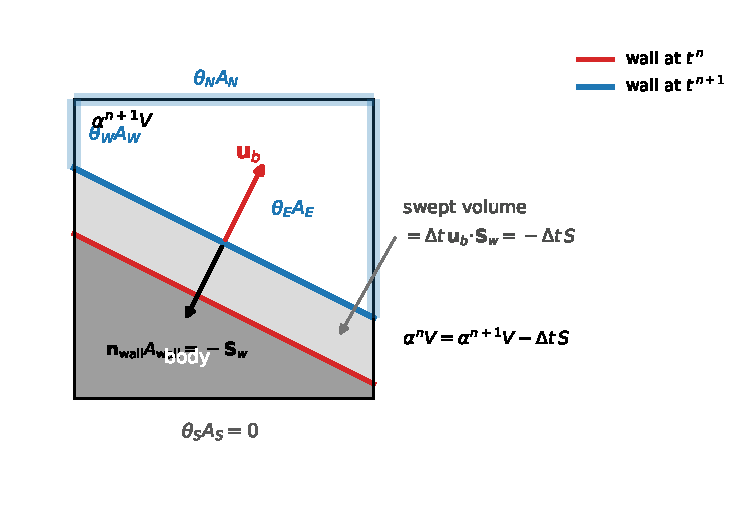
\includegraphics[width=0.62\textwidth]{figs3/f1_swept.pdf}
\caption{A cut cell over one step. The axis faces are fixed in space; only their wet fractions
$\theta_f$ change. The shaded band is the volume the wall sweeps, which is
$-\dt\,S_P=\dt\,\ub\!\cdot\!\Sw$ and is the \emph{only} quantity the motion contributes to the
discretisation.}
\label{fig:swept}
\end{figure}

\subsection{Continuity is the only equation that changes}

Table~\ref{tab:terms} lists every term against its stationary counterpart.

\begin{table}[t]
\centering
\small
\begin{tabular}{@{}lll@{}}
\toprule
term & body at rest & body moving \\
\midrule
continuity & $\sum_f\theta_f\phi_f=0$ & $\sum_f\theta_f\phi_f=\ub\!\cdot\!\Sw$ \\
convective & no wall term & no wall term \\
pressure & $p_P\nn_{\rm wall}A_{\rm wall}$, absorbed by \eqref{eq:closure} & same \\
viscous, free slip & no wall term & no wall term \\
viscous, no slip & $\nu(0-u_P)A_{\rm wall}/d$ & $\nu(u_b-u_P)A_{\rm wall}/d$ \\
unsteady & $\alpha_P V(u^{n+1}-u^{n})/\dt$ & $(\alpha^{n+1}u^{n+1}-\alpha^{n}u^{n})V/\dt$ \\
\bottomrule
\end{tabular}
\caption{Every term of the discretisation. Only the first and the last two rows differ, and the
convective row is the one that is easy to get wrong.}
\label{tab:terms}
\end{table}

The convective row deserves a word. The absolute mass flux through the wall is not zero, so one
might expect a wall term $\uu(\uu\!\cdot\!\nn)A_{\rm wall}$. Writing the momentum balance over
the \emph{time-varying} region $\Omega_P(t)$ removes it: the flux that appears there is the
relative one, $\uu(\uu-\bm{w})\!\cdot\!\nn$ with $\bm{w}$ the velocity of the boundary, and on the
wall $\bm{w}=\ub$ and $(\uu-\ub)\!\cdot\!\nn=0$. On the axis faces $\bm{w}=\bm{0}$ and the flux is
the absolute one, exactly as in the stationary case. So the convective operator is untouched --
provided the unsteady term is the one in Table~\ref{tab:terms}, with the volume inside the
difference.

\subsection{Free slip needs nothing added}

In the stationary method, no-penetration is not imposed anywhere: it \emph{emerges}. For a
uniform $\bm{c}$ in a cut cell, closure gives $\sum_f\theta_f\bm{c}\!\cdot\!\nn_fA_f=
\bm{c}\!\cdot\!\Sw$, and setting this to zero forces $\bm{c}\!\cdot\!\nn_{\rm wall}=0$.

The same argument runs unchanged on a moving wall. Setting
$\bm{c}\!\cdot\!\Sw=\ub\!\cdot\!\Sw$, which is what \eqref{eq:continuity} demands, forces
\begin{equation}
\bm{c}\!\cdot\!\nn_{\rm wall}=\ub\!\cdot\!\nn_{\rm wall}.
\end{equation}
The moving-wall no-penetration condition is a consequence of discrete continuity plus closure,
and \emph{the mass source is the boundary condition}. Nothing else is added for free slip: no
ghost value, no extrapolation, no velocity coupling.

\subsection{No slip adds one source}

The wall traction of a no-slip wall moving at $\ub$ is
\begin{equation}
\int_{\rm wall}\!\nu\,\frac{\partial \uu}{\partial n}\dd S
\;\simeq\;\nu\,\frac{\ub-\uu_P}{d}\,A_{\rm wall},
\qquad d=\frac{\alpha_P V}{2A_{\rm wall}},
\label{eq:noslip}
\end{equation}
$d$ being the mean thickness of the fluid the cell holds behind its wall segment, halved for a
profile linear in the wall-normal direction. The $\uu_P$ half is the diagonal term of the
stationary scheme, unchanged: the body velocity does not enter it. The $\ub$ half is a source.
It vanishes for a wall at rest, which is why the stationary formulation needs no source at all.

Because $d\propto\alpha_P$, the coefficient $\nu A_{\rm wall}/d$ grows like $1/\alpha_P$ as a
cell is squeezed against the wall. The small-cell limit therefore \emph{strengthens} diagonal
dominance and drives $\uu_P\to\ub$, rather than degrading the system --- the same property the
stationary scheme has, now pulling the cell onto the moving wall instead of onto rest.

\section{Which quantity is primary}
\label{sec:primary}

Equations \eqref{eq:volume} and \eqref{eq:continuity} are the same statement, so on paper one may
take either as the definition and derive the other. Discretely the two choices are not
equivalent, and only one of them works.

\subsection{The two candidates}

\paragraph{Candidate A: geometry first.} Compute $\alpha^{n}$ and $\alpha^{n+1}$ from the level
set and set
\begin{equation}
S_P = \frac{(\alpha^{n+1}_P-\alpha^{n}_P)V}{\dt}.
\label{eq:candA}
\end{equation}
This is the textbook swept-volume prescription and it is what one writes down first.

\paragraph{Candidate B: flux first.} Compute $\Sw$ from $\theta^{n+1}$ and set
\begin{equation}
S_P = -\,\ub\!\cdot\!\Sw,
\qquad\text{then}\qquad
\alpha^{n}_P V := \alpha^{n+1}_P V-\dt\,S_P .
\label{eq:candB}
\end{equation}

\subsection{Why A fails}

Candidate A presumes that $\alpha$ can be differentiated in time. It cannot, because $\alpha$ is
not known exactly: \texttt{cellFraction} obtains it by sub-sampling the level set, with an error
of order $10^{-3}$ per cell at $32\times32$ samples. Dividing that error by $\dt$ amplifies it
without bound. Table~\ref{tab:AB} compares the two candidates directly for a cylinder translating
at $u_b=0.37$ on an $81^2$ mesh.

\begin{table}[t]
\centering\small
\begin{tabular}{@{}lrrr@{}}
\toprule
$\dt$ & displacement & $\max|S_A-S_B|/\max|S_B|$ & $\sum_P S_{A,P}$ \\
\midrule
0.2000 & 0.599 cells & 0.890 & $+4.5\times10^{-4}$\\
0.1000 & 0.300 cells & 0.199 & $-3.0\times10^{-3}$\\
0.0500 & 0.150 cells & 0.280 & $-3.6\times10^{-3}$\\
0.0250 & 0.075 cells & 0.561 & $-1.2\times10^{-3}$\\
0.0125 & 0.037 cells & 0.166 & $+3.1\times10^{-2}$\\
\bottomrule
\end{tabular}
\caption{Candidate A against candidate B. The difference does not converge as $\dt\to0$ --- it
is quadrature noise divided by $\dt$ --- and $\sum_P S_{A,P}$, which must vanish, does not.
For candidate B, $\sum_P S_{B,P}$ is $10^{-17}$ at every row.}
\label{tab:AB}
\end{table}

The last column is the more serious failure. The fluid region is a pure Neumann island for the
pressure, so the pressure system is singular and needs a reference; following
\texttt{fvMatrix::setReference} the reference is imposed by \emph{doubling} one diagonal entry
rather than by replacing a row, which keeps the matrix symmetric. As shown in
\S\ref{sec:compat}, that construction returns the true solution \emph{only} if the right-hand
side is compatible. Candidate A is not compatible, so the entire mismatch is deposited in the
reference cell as a spurious point mass source. Projecting the residual away restores
solvability but leaves an $O(10^{-3})$ spurious dilatation, and the measured free-stream error
of the resulting scheme is $50\%$ of $u_b$.

\subsection{Why B works}

Candidate B never differentiates a sampled quantity. Two properties come free.

\begin{proposition}[Exact compatibility]
$\sum_P S_P=0$ to roundoff, for every body position, every body velocity and every pattern of
absorbed slivers.
\end{proposition}
\begin{proof}
$S_P=-\ub\!\cdot\!\Sw$ with $\Sw=\sum_f\theta_f\nn_fA_f$. Summing over all cells, each interior
face appears twice with opposite normals and identical $\theta$, so the sum telescopes; the
periodic seam contributes nothing because $\theta$ there is computed once and copied. An absorbed
sliver has all its faces closed, so $\Sw=\bm{0}$ and it contributes nothing at all.
\end{proof}

\begin{proposition}[Exactness for the divergence operator]
For a uniform $\uu\equiv\ub$, $\operatorname{div}\phi=\ub\!\cdot\!\Sw=-S$ identically.
\end{proposition}
\begin{proof}
$\Sw$ is assembled from exactly the $\theta$ that \texttt{interpolatePhi} multiplies the face
velocities by. The two expressions are the same sum.
\end{proof}

The second half of \eqref{eq:candB}, $\alpha^{n}V:=\alpha^{n+1}V-\dt S$, is a backward Euler
integration of the volume ODE~\eqref{eq:volume}. It is the classical resolution of the
geometric conservation law --- \emph{take the volume from the flux, not the flux from the
volume} --- applied per step. Because $\alpha^{n}$ is recomputed from the current geometry every
step and never accumulated, it cannot drift.

\section{The discrete geometric conservation law}

\begin{proposition}[Free-stream preservation]
Let the body translate rigidly at $\ub$ and let $\uu^{n}\equiv\ub$ throughout the domain, with
$p\equiv0$. Then $\uu^{n+1}\equiv\ub$, $p\equiv0$ is an exact solution of the discrete system,
for any $\dt$, any body path, any mesh, and either wall condition.
\end{proposition}

\begin{proof}
Take the momentum row of a fluid cell $P$ and apply the operator to the constant field $\ub$.
The row sum of each contribution is:
\begin{itemize}\itemsep2pt
\item unsteady: $\alpha^{n+1}V/\dt$;
\item convective: the \texttt{fvm\_divConvFlux} stencil has row sum
      $\phi_E-\phi_W+\phi_N-\phi_S=\operatorname{div}\phi=-S$;
\item viscous: the $\theta$-weighted Laplacian has row sum zero, so it annihilates a constant,
      as it must;
\item no-slip wall: diagonal $+\nu A_{\rm wall}/d$, matched on the right-hand side by
      $+\nu A_{\rm wall}\ub/d$ from \eqref{eq:noslip}; they cancel at $\uu_P=\ub$;
\item pressure: \texttt{fvc\_grd} is written through \eqref{eq:closure} as
      $\sum_f\theta_f(p_f-p_P)\nn_fA_f$ and vanishes for uniform $p$.
\end{itemize}
The equation therefore reduces to
\begin{equation}
\left(\frac{\alpha^{n+1}V}{\dt}-S\right)\ub \;=\; \frac{\alpha^{n}V}{\dt}\,\ub ,
\end{equation}
which is precisely the definition \eqref{eq:candB} of $\alpha^{n}$. Continuity is satisfied
because $\operatorname{div}\phi=-S$ identically for the uniform field (Proposition 2), so the
pressure equation has zero right-hand side and $p\equiv 0$ solves it.
\end{proof}

\begin{remark}[The effective unsteady diagonal]
The \emph{diagonal} contribution of the convective operator is $\tfrac12\operatorname{div}\phi$,
so unsteady and convective terms contribute
$\alpha^{n+1}V/\dt-\tfrac12 S=\tfrac12(\alpha^{n+1}+\alpha^{n})V/\dt$ to the diagonal: the
\emph{average} of the old and new fluid volume. A cell emerging from the body, with
$\alpha^{n}=0$, still carries half its new volume on the diagonal and cannot lose positivity for
that reason.
\end{remark}

\subsection{Compatibility and the doubled reference diagonal}
\label{sec:compat}

Let $L$ be the pressure matrix restricted to the fluid cells, so that $\bm{1}^{\!\top}L=\bm{0}$
(a Laplacian assembled from face fluxes has columns summing to zero, and solid cells decouple
because all their faces are closed). The reference is imposed as
$L'=L+\bm{e}_r\bm{e}_r^{\!\top}d_r$ with $d_r=L_{rr}$.

Suppose $\bm{1}^{\!\top}\bm{b}=0$ and let $p$ solve $L'p=\bm{b}$. Then
$Lp=\bm{b}-\bm{e}_rd_rp_r$, and left-multiplying by $\bm{1}^{\!\top}$ gives $d_rp_r=0$, hence
$p_r=0$ and $Lp=\bm{b}$ exactly. The doubled diagonal is therefore \emph{transparent} for a
compatible right-hand side: it selects the solution that vanishes at the reference cell, and
perturbs nothing.

For an incompatible right-hand side the same algebra gives $d_rp_r=\bm{1}^{\!\top}\bm{b}\ne0$,
and the whole defect appears as a point source at the reference cell. This is why exact
compatibility, and not merely small incompatibility, is the property that matters --- and why
candidate B, which has it by construction, is preferable to candidate A plus a projection.

\section{Algorithm}

\subsection{Where the source enters}

The step is a PIMPLE-style loop: the geometry is advanced once, then held fixed while
$n_{\rm outer}$ SIMPLEC iterations converge the nonlinearity.

\begin{enumerate}\itemsep2pt
\item Move the body to $t+\dt$ and rebuild $\theta$, $\alpha$, $\Sw$, $A_{\rm wall}$, $d$ and the
      fluid/solid mask.
\item Form $S=-\ub\!\cdot\!\Sw$ and $\alpha^{n}V=\alpha^{n+1}V-\dt S$.
\item Assemble the step-invariant sources: $\alpha^{n}V\uu^{n}/\dt$, the no-slip wall source
      $\nu A_{\rm wall}\ub/d$, and the blanking source that drives the solid interior to $\ub$.
\item For each outer iteration: assemble the momentum operators, solve the predictor, form
      $\uu_{HbyA}$ and $\phi_{HbyA}$, and solve
      \begin{equation}
      \nabla\!\cdot\!\big(r_{A_tU}V\,\nabla p\big)=\nabla\!\cdot\!\phi_{HbyA}+S ,
      \label{eq:poisson}
      \end{equation}
      then correct $\phi=\phi_{HbyA}-r_{A_tU}V\nabla p$ so that
      $\nabla\!\cdot\!\phi=-S$.
\end{enumerate}
Equation \eqref{eq:poisson} is the entire algorithmic modification: one added term on the
right-hand side of the pressure equation.

\subsection{Constant flow rate}

A doubly periodic box leaves the mean flow undetermined, so it must be pinned. The solver does so
by superposition: the whole pass is affine in $(\text{source},p^{\rm old},S)$, so one pass with
$g_x=0$ and one with $g_x=1$ give the exact $g_x$ that lands the bulk velocity on its target,
with no gain to tune. The moving-wall contributions --- $S$, the wall source, the blanking
source --- all belong to the $g_x=0$ problem, so the superposition is untouched by them. Setting
the target to zero is the natural choice for a body stirring an otherwise quiescent fluid, and is
what makes the reported force meaningful.

\subsection{Re-interpolating the flux across a geometry change}
\label{sec:reinterp}

One line does not follow from the formulation but matters as much as any of it. The flux
$\phi^{n}$ carried from the previous step lives on the faces of the \emph{old} cut mesh: a face
that has just opened has no history there, and one that has just closed carries a history that no
longer exists. Before the outer loop starts, $\phi$ is therefore re-interpolated from $\uu^{n}$
through the \emph{new} $\theta$.

Nothing is lost: this is only the initial guess for the convective operator, and the flux the
step returns is the Rhie--Chow projected one either way. What is gained is that for a fluid
translating rigidly with the body the guess lands \emph{exactly} on the fixed point, so
free-stream preservation is exact from the first outer iteration. Without it the fixed point is
still exact but is only approached at roughly a factor of two per outer iteration, which costs
two to four digits at practical $n_{\rm outer}$ --- see Table~\ref{tab:freestream}.

\section{Verification}

\subsection{Free-stream preservation}

Fill the domain with $\uu=\ub$ and translate the body at that velocity. The fluid moves rigidly
with the body: no relative motion, no pressure gradient, no traction, so $\uu\equiv\ub$ is the
exact solution and any departure is a discretisation error. The test exercises the two-level
unsteady term, the mass source, the moving-wall traction and the blanking simultaneously, and a
sign error in any of them gives an $O(1)$ result.

\begin{table}[h]
\centering\small
\begin{tabular}{@{}lrrrr@{}}
\toprule
& \multicolumn{4}{c}{$\max|\uu-\ub|$ after 5 steps} \\
\cmidrule(l){2-5}
$n_{\rm outer}$ & 1 & 2 & 3 & 5\\
\midrule
$u_b=0.37$, with \S\ref{sec:reinterp}    & 5.6e-16 & 5.6e-16 & 5.6e-16 & 6.1e-16\\
$u_b=2.00$, with \S\ref{sec:reinterp}    & 3.6e-15 & 4.0e-15 & 3.6e-15 & 3.6e-15\\
\midrule
$u_b=0.37$, without \S\ref{sec:reinterp} & 1.6e-03 & 1.4e-04 & 6.9e-05 & 2.4e-05\\
$u_b=2.00$, without \S\ref{sec:reinterp} & 1.2e-01 & 1.2e-02 & 6.5e-03 & 2.5e-03\\
\midrule
$u_b=0.37$, candidate A of \S\ref{sec:primary} & 6.8e-02 & 6.3e-02 & 6.0e-02 & 5.6e-02\\
$u_b=2.00$, candidate A of \S\ref{sec:primary} & 1.8e+00 & 1.8e+00 & 1.9e+00 & 1.9e+00\\
\bottomrule
\end{tabular}
\caption{Free-stream preservation, $n_x=81$, $\nu=1$, $\dt=0.025$, no slip. Machine precision at
any body speed and from the first outer iteration. Candidate A does not converge with
$n_{\rm outer}$ at all: its error is not a splitting error but a wrong fixed point.}
\label{tab:freestream}
\end{table}

\subsection{Mass conservation}

Over an oscillating-cylinder run, $\max_P|\operatorname{div}\phi+S|\sim10^{-16}$ and
$|\sum_P(\operatorname{div}\phi+S)|\sim10^{-17}$ at every step, including steps in which slivers
are absorbed or released. No projection is applied anywhere. See the bottom panel of
Fig.~\ref{fig:history}.

\subsection{Consistency of the swept volume}

$\alpha^{n}V=\alpha^{n+1}V-\dt S$ is a backward Euler integration of \eqref{eq:volume}, so it
must converge to the geometric $\alpha$ at the old time. Table~\ref{tab:swept} confirms it. The
comparison is restricted to cells that are cut in both configurations, since a cell crossing the
sliver threshold in between changes by \texttt{ALPHA\_MIN} for reasons unrelated to the time
integration.

\begin{table}[h]
\centering\small
\begin{tabular}{@{}lrrr@{}}
\toprule
$\dt$ & mean $|\alpha^{n}-\alpha_{\rm geom}|$ & order & cells with $\alpha^{n}<0$\\
\midrule
0.4000 & 2.565e-01 & --- & 17\\
0.2000 & 8.638e-02 & 1.6 & 12\\
0.1000 & 2.260e-02 & 1.9 & 2\\
0.0500 & 9.147e-03 & 1.3 & 0\\
0.0250 & 3.099e-03 & 1.6 & 0\\
0.0125 & 1.347e-03 & 1.2 & 0\\
\bottomrule
\end{tabular}
\caption{The swept volume against the geometry, $u_b=0.37$, $n_x=81$. The exactness of
Table~\ref{tab:freestream} is not bought by evolving a volume that has come loose from the body.}
\label{tab:swept}
\end{table}

\subsection{Galilean invariance}

A fixed body in a bulk flow $+U$ and a body translating at $+U$ through a fluid of zero bulk
velocity differ by a Galilean shift, so the streamwise forces must satisfy $F^{\rm mov}_x=
-F^{\rm fix}_x$. The two are computed through entirely different terms --- the moving case
exercises the mass source, the wall source and the two-level unsteady term, none of which the
fixed case touches --- so the comparison is an independent check of the whole construction.
\begin{table}[h]
\centering\small
\begin{tabular}{@{}lrr@{}}
\toprule
configuration & $F_x$ & ripple \\
\midrule
fixed body, bulk velocity $+U$  & $+5.66034$ & $\pm0.00000$ \\
body at $+U$, bulk velocity $0$ & $-5.69040$ & $\pm0.15625$ \\
\midrule
relative difference & \multicolumn{2}{r}{$0.53\%$} \\
\bottomrule
\end{tabular}
\caption{Galilean invariance. $U=0.5$, $\nu=1$, $n_x=81$, $\dt=0.025$, no slip; each case run to
$t=30$ and averaged over the last $400$ steps. The moving case carries a ripple of $\pm2.8\%$ at
the frequency $U/h$ at which the body slides from one cut pattern to the next --- the
characteristic signature of a non-body-fitted cut-cell method, and the same effect that makes the
cylinder drag a poor instrument for measuring the order of convergence. The means agree to well
inside it.}
\label{tab:galilean}
\end{table}


\subsection{Physical behaviour}

Figures~\ref{fig:field} and~\ref{fig:history} show a cylinder oscillating along $x$ in an
otherwise quiescent periodic box, no slip, $\nu=1$, $n_x=81$. The impulsive start produces the
expected added-mass spike; thereafter the force follows the body velocity with the phase lag of a
viscous flow, and the bulk velocity stays at its target of zero to $10^{-18}$.

\begin{figure}[t]
\centering
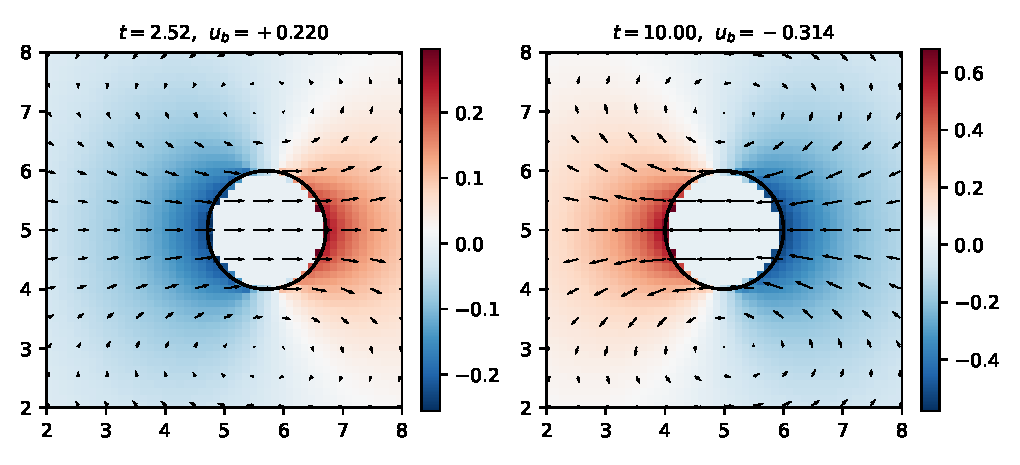
\includegraphics[width=\textwidth]{figs3/f2_field.pdf}
\caption{Pressure and velocity around the oscillating cylinder at two instants.}
\label{fig:field}
\end{figure}

\begin{figure}[t]
\centering
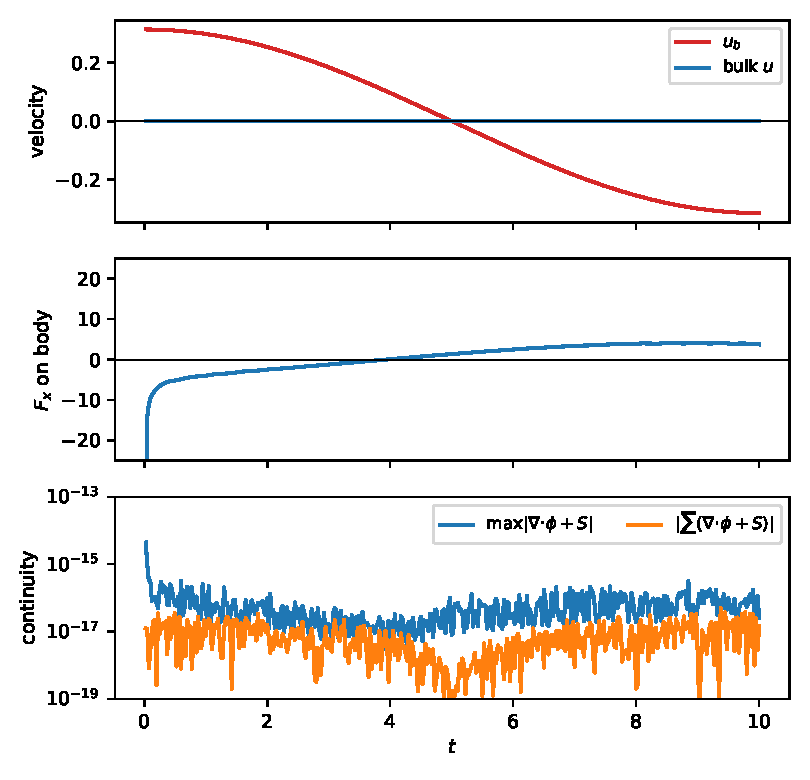
\includegraphics[width=0.72\textwidth]{figs3/f3_history.pdf}
\caption{Oscillating cylinder: body and bulk velocity, streamwise force, and the two continuity
diagnostics. The force axis is clipped; the impulsive start reaches $-60$.}
\label{fig:history}
\end{figure}

\section{Step restriction}

The row sum of the unsteady plus convective operator is exactly $\alpha^{n}V/\dt$, so it changes
sign when $\alpha^{n}$ does. From \eqref{eq:candB},
\begin{equation}
\alpha^{n}_P V=\alpha^{n+1}_P V+\dt\,\ub\!\cdot\!\Sw
\quad\Longrightarrow\quad
\boxed{\;\dt\,|\ub| \;\lesssim\; \frac{\alpha_P V}{A_{\rm wall}}\;=\;2d\;}
\label{eq:cfl}
\end{equation}
The wall must not sweep through more than a wall-adjacent cell holds. Three things follow.

\begin{itemize}\itemsep3pt
\item It is a condition on the \emph{smallest wet cell}, not on the mesh spacing. Refining the
      mesh does not tighten it in any simple way; \texttt{ALPHA\_MIN}, which sets the smallest
      $\alpha$ admitted, does.
\item It is not fatal when violated in a few cells. The diagonal there is still dominated by the
      viscous and wall terms, which grow like $1/\alpha_P$; what is lost is positivity of the
      row sum, not of the matrix. Runs with two or three violating cells out of $6380$ are
      indistinguishable from clean ones. A large count means the step is genuinely too big.
\item The solver reports $\min_P\alpha^{n}_P$ and the number of violating cells at every step.
\end{itemize}

\section{Limitations}

\paragraph{First order in time.} Implicit Euler, and the volume integration in
\eqref{eq:candB} inherits it. A second-order extension (BDF2) needs $\alpha$ at three levels and
a three-level form of the argument in \S4; the structure carries over but the bookkeeping does
not, since $\alpha^{n-1}$ would then have to be stored rather than reconstructed.

\paragraph{First order in space for no slip.} Unchanged from the stationary method: free slip is
second order because it needs no wall-normal distance, no slip is first order because the
estimate $d=\alpha_PV/(2A_{\rm wall})$ is first-order accurate. Measured $L_2$ orders on a curved
wall are $2.21, 2.33, 2.06, 2.14$ (free slip) against $0.75, 1.27, 0.91, 0.90$ (no slip).

\paragraph{Absorbed slivers lose their content.} A cell crossing \texttt{ALPHA\_MIN} is
deactivated and hands over no momentum, an $O(\texttt{ALPHA\_MIN}\cdot V)$ defect and the same
one the stationary method has. Mass conservation is \emph{not} affected: an absorbed cell has all
faces closed, hence $\Sw=\bm{0}$, hence no source and no contribution to the compatibility sum.
Cell merging rather than absorption is the clean fix and would also relax \eqref{eq:cfl}.

\paragraph{Prescribed motion.} The hydrodynamic force is available --- the pressure part is
$-\sum_P p_P\Sw$ by \eqref{eq:closure}, and the viscous part is the reaction to the traction
already assembled in \eqref{eq:noslip} --- so closing a rigid-body ODE is short. A light body
would need the added-mass sub-iteration inside the outer loop.

\paragraph{One fluid region.} The pressure reference is a single cell, chosen as the fluid cell
farthest from the body so that the body cannot swallow it. Should the body ever split the fluid
in two, one reference per region would be required.

\section{Summary}

A rigid body moving through a fixed cut-cell mesh changes exactly one equation. Continuity
acquires the source $S=-\ub\!\cdot\!\Sw$, and that source is simultaneously the moving-wall
no-penetration condition, so free slip needs nothing else and no slip needs only the $\ub$ half
of its wall traction.

The choice that decides whether the scheme works is which of the volume change and the wall flux
is primary. Taking the flux as primary and the volume change from it gives exact compatibility of
the pressure system, exact consistency with the divergence operator, and a discrete geometric
conservation law that holds by construction; the reverse ordering differentiates a sampled
volume and fails outright. With one further line --- re-interpolating the carried flux onto the
new geometry --- a free stream is preserved to machine precision at any body speed and from the
first outer iteration, and mass is conserved to roundoff without any projection.

\end{document}
